% SVN info for this file
\svnidlong
{$HeadURL$}
{$LastChangedDate$}
{$LastChangedRevision$}
{$LastChangedBy$}

\chapter{Varietà topologiche}
\labelChapter{varietà}

\begin{introduction}
	‘‘BEEP BOOP INSERIRE CITAZIONE QUA BEEP BOOP.''
	\begin{flushright}
		\textsc{NON UN ROBOT,} UN UMANO IN CARNE ED OSSA BEEP BOOP.
	\end{flushright}
\end{introduction}

\section{Varietà topologiche}
%AAA INTRODUZIONE BELLA CERCASI
Si vuole formalizzare il concetto di avere \textit{localmente} la topologia euclidea. 
%BIBLIOGRAFIA
\begin{define}\textsc{Localmente euclideo.}\\
	Uno spazio topologico $X$ si dice \textbf{localmente euclideo}\index{localmente euclideo} di dimensione $n$ se ogni punto di $X$ ammette un intorno aperto omeomorfo ad una palla aperta di $\realset^n$.
\end{define}

\begin{define}\textsc{Varietà topologica.}\\
	Uno spazio topologico $X$ si dice \textbf{varietà topologica}\index{varietà topologica} di dimensione $n$ se $X$ è di \textbf{Hausdorff}, connesso, a base numerabile e localmente euclideo di dimensione $n$.
\end{define}

\begin{examples}
	\begin{itemize}
		\item $\realset^n$ è una varietà topologica di dimensione $n$.
		\item $S^n$ è una varietà topologica compatta di dimensione $n$, infatti grazie alla proiezione stereografica si ha che $S^\setminus\{*\}\cong \realset$.
		\item $\mathbb{P}^n(\realset)$ è una varietà topologica compatta di dimensione $n$.
		\item Ogni aperto connesso di una varietà topologica di dimensione $n$ è una varietà topologica di dimensione $n$.
	\end{itemize}
\vspace{-3mm}
\end{examples}
\begin{observe}
	La dimensione di una varietà topologica è \textit{ben definita} per l'\textit{invarianza della dimensione}.
\end{observe}
\begin{observes}~{}
	\begin{itemize}
		\item Una varietà topologica è \textbf{c.p.a.}.
		\item Se $X$ è una varietà topologica di dimensione $n$ e $Y$ è una varietà topologica di dimensione $m$ allora $X\times Y$ è una varietà topologica di dimensione $n+m$.
	\end{itemize}
%DIMOSTRAZIONE TUTORATO dei due punti precedenti
\end{observes}
\begin{example}
	$T=S^1\times S^1$ è una varietà topologica di dimensione $2$.
\end{example}

\begin{theorema}
	Sia $X$ uno spazio topologico compatto, connesso, \textbf{Hausdorff} e localmente euclideo di dimensione $n$. Allora $X$ è a \textit{base numerabile}, dunque $X$ è una varietà topologica di dimensione $n$.
\end{theorema}
 
\subsection{Dimensione 1}
Analizziamo il caso di varietà topologiche di dimensione $1$, per esempio $\realset$ e $S^1$.
\begin{theorema}
	Ogni varietà topologica di dimensione $1$ è omeomorfo a $\realset$ se \textit{non} è compatta, oppure a $S^1$ se compatta.
\end{theorema}
\begin{example} 
Riconsideriamo l'esempio della \textbf{retta con 2 origini} (sez. \ref{retta 2 origini}, pag. \ref{retta 2 origini}): essa è un quoziente non \textbf{Hausdorff}, dunque \textit{non} è una varietà topologica.
\end{example}
	\subsection{Dimensione 2}
\begin{define}\textsc{Superficie topologica.}\\
	Una varietà topologica di dimensione $2$ si dice \textbf{superficie topologica}\index{superficie!topologica}.
\end{define}
\begin{examples}
	\begin{itemize}
		\item Il \textit{piano} $\realset^2$ oppure $\realset^2\setminus \{n\text{ punti}\}$ sono superfici topologiche di dimensione $2$ \textit{non} compatte.
		\item La \textbf{sfera} $S^2$ è una superficie topologica compatta.
		\item Il \textbf{toro} $T=S^1\times S^1$ è una superficie topologica compatta.
		\item Il \textbf{piano proiettivo} $\mathbb{P}^2(\realset)$ una superficie topologica compatta.
	\end{itemize}
\vspace{-3mm}
\end{examples}
Vogliamo dare una classificazione delle superfici topologiche \textit{compatte}. Innanzitutto, esaminiamo alcuni esempi di superfici compatte studiandole sul \textit{modello piano}, di cui daremo successivamente una definizione formale.
\begin{examples} \textsc{Modelli piani.}\\
			\begin{itemize}
		\item Siccome $\mathbb{P}^2(\realset)$ è un quoziente del disco, allora, a meno di omeomorfismo, lo si può anche vedere come un quoziente di $I\times I$ con una relazione di equivalenza sul bordo con \textit{parola} $abab$.
		\begin{center}
		\includegraphics[trim=0cm 0cm 0cm 0cm, clip, scale=0.375]{images/proj.pdf}
		\end{center}
		\item Anche il \textbf{toro} si può vedere come quoziente di $I\times I$ con \textit{parola} $aba^{-1}b^{-1}$.
		\begin{center}
			\includegraphics[trim=0cm 0cm 0cm 0cm, clip, scale=0.375]{images/torus.pdf}
		\end{center}
		\item Vediamo $S^2$ come quoziente di $I\times I$ con \textit{parola} $bb^{-1}a^{-1}a$.
		\begin{center}
			\includegraphics[trim=0cm 0cm 0cm 0cm, clip, scale=0.375]{images/sphere.pdf}
		\end{center}
	\end{itemize}
\vspace{-6mm}
\end{examples}

\begin{observe}
	Sia $P\subset\realset^2$ un \textit{poligono} pieno con un numero \textit{pari} di lati. Sia $\sim$ una relazione di equivalenza che identifica i lati a $2$ a $2$. Allora $S\coloneqq\nicefrac{P}{\sim}$ è una \textit{superficie topologica compatta}, infatti:
		\begin{enumerate}
			\item  $P$ è connesso e compatto $\implies S$ connesso e compatto.
			\item $S$ è localmente euclideo di dimensione $2$. Sia $p\in S$, se $p$ viene da un punto interno al poligono allora si sceglie un intorno aperto $U$ centrato in tale punto tale che $U\cap\partial{P}=\emptyset$, data la proiezione $\funz \pi P S$, $\pi(U)\cong U$ ed è un intorno aperto di $p$. Se $p$ viene da un punto interno ad un lato grazie all'identificazione dei lati a due a due si ha che passando al quoziente, cioè un intorno aperto di $p$ omeomorfo ad un disco aperto. Se $p$ viene da un vertice, siccome i vertici vengono identificati con i vertici, analogamente al caso dei lati si ottiene un intorno aperto di $p$ in $S$ omeomorfo ad un disco aperto di $\realset^2$.
			\item $S$ è di \textbf{Hausdorff}.
		\end{enumerate}
	% riguardare la frase, magari separare in un equazione a parte
	Osserviamo che nella relazione di equivalenza due lati vengono identificati nel modo seguente: $l_i\cong\intv$, dunque scelgo un omeomorfismo $l_1\stackrel{\stackrel{\phi}{\sim}}{\longrightarrow} l_2$, $p_1\in l_1 \sim \phi(p)\in l_2$ e $\phi$ manda vertici in vertici.\\
	Il poligono $P$ con la relazione di equivalenza sui lati è detto un \textbf{modello piano}\index{modello piano} della superficie $S$ e può essere schematizzato con una \textit{sequenza di lettere} detta \textbf{parola}\index{parola}. Ad esempio, per la parola $aba^{-1}cbc^{-1}$ si ottiene il modello piano seguente:
		\begin{center}
	\includegraphics[trim=0cm 0cm 0cm 0cm, clip, scale=0.375]{images/modellopiano.pdf}
\end{center}
 Inoltre, il modello piano di una superficie compatta \textit{non è unico}.
\end{observe}

\begin{examples}
	\begin{itemize}
		\item Abbiamo già visto il modello piano di $S^2$ sul \textit{quadrato}; per la costruzione effettuata, possiamo unire la sequenza di lati $ab$ in un unico lato $c$ in modo da ottenere un modello costituito da un poligono \textit{improprio a due lati}, con parola $cc^{-1}$:
		\begin{center}
			\includegraphics[trim=0cm 0cm 0cm 0cm, clip, scale=0.375]{images/sphere2lines.pdf}
		\end{center}
		\item Anche il modello piano di $\mathbb{P}^2(\realset)$ sul \textit{quadrato} può essere trasformato in uno sul poligono a due lati, unificando $ba$ per ottenere un'unico lato $c$ e un modello con parola $cc$:
		\begin{center}
			\includegraphics[trim=0cm 0cm 0cm 0cm, clip, scale=0.375]{images/proj2lines.pdf}
		\end{center}
		\item La \textbf{bottiglia di Klein}\index{bottiglia di Klein} $K$ è la superficie compatta data dal modello piano:
				\begin{center}
			\includegraphics[trim=0cm 0cm 0cm 0cm, clip, scale=0.375]{images/klein.pdf}
		\end{center}
		Confrontiamo la costruzione della bottiglia di Klein con la costruzione del \textit{toro}, vista precedentemente. Innanzitutto otteniamo in entrambi il cilindro $S^1\times I$ con la relazione di equivalenza sul \textit{bordo}; notiamo che nella bottiglia di Klein (il modello inferiore nella figura sotto) il ‘‘verso'' rispetto al quale \textit{incolleremo} i bordi sono uno l'opposto dell'altro.
		\begin{center}
			\includegraphics[trim=0cm 0cm 0cm 0cm, clip, scale=0.375]{images/kleintorus.pdf}
		\end{center}
	Questo comporta che la bottiglia di Klein \textit{non} può essere rappresentata in $\realset^3$; tuttavia, possiamo visualizzarla in modo improprio operando un ‘‘\textit{taglio}'' nella superficie e compenetrando uno dei due estremi del cilindro nella figura, come di seguito.
	 \begin{center}
	 	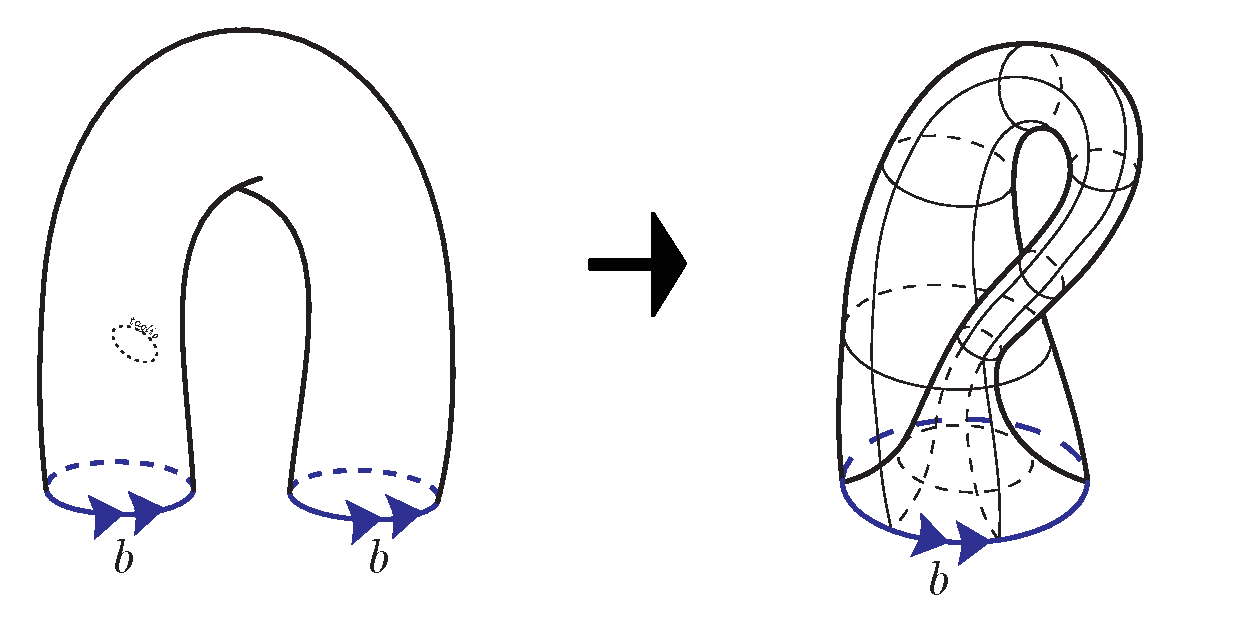
\includegraphics[trim=0cm 0cm 0cm 0cm, clip, scale=0.375]{images/kleinconstruction.pdf}
	 \end{center}
	\end{itemize}
\end{examples}

	\subsection{Somma connessa}
Siano $S_1$ e $S_2$ superfici compatte e siano $x\in S_1$ e $y\in S_2$. Siano $D_x\subset S_1$ e $D_y\subset S_2$ intorni di $x$ e $y$ rispettivamente, omeomorfi ad un disco chiuso $D\subset\realset^2$:
% https://q.uiver.app/?q=WzAsMixbMCwwLCJEX3giXSxbMSwwLCJEX3kiXSxbMCwxLCJcXHN0YWNrcmVse2h9e1xcc2ltfSJdXQ==
\[\begin{tikzcd}
	{D_x} & {D_y}
	\arrow["{\stackrel{h}{\sim}}", from=1-1, to=1-2]
\end{tikzcd}\]
\begin{center}
	\includegraphics[trim=0cm 0cm 0cm 0cm, clip, scale=0.4]{images/connectedsum1.pdf}
\end{center}
\textit{Togliamo} dalle due superfici gli interni dei dischetti, creando dunque lo spazio:
\begin{equation*}
	Y\coloneqq (S_1\setminus \interior{D_x})\amalg (S_2\setminus \interior{D_y})
\end{equation*}
\begin{center}
	\includegraphics[trim=0cm 0cm 0cm 0cm, clip, scale=0.4]{images/connectedsum2.pdf}
\end{center}
\textit{Incolliamo} ora i due pezzi di $Y$ lungo i bordi dei dischi, cioè mettiamo su $Y$ la seguente relazione di equivalenza:
\begin{equation*}
	x_1\sim y_1 \iff x_1=y_1\text{ oppure } x_1\in\partial{D},\ y_1\in\partial{D}\text{ e } y_1=h(x_1)\text{ (o viceversa)} 
\end{equation*}
\begin{center}
	\includegraphics[trim=0cm 0cm 0cm 0cm, clip, scale=0.4]{images/connectedsum3.pdf}
\end{center}
Vediamo ora qualche fatto che \textit{non} dimostriamo:
	\begin{itemize}
		\item Il quoziente è ancora una superficie topologica, che chiamiamo \textbf{somma connessa}\index{somma!connessa} $S_1\# S_2$  di $S_1$ e $S_2$. 
		\item La somma connessa $S_1\# S_2$, a meno di omeomorfismo, \textit{non dipende} dalle scelte fatte come i punti $x$ e $y$, gli intorni $D_x$ e $D_y$, l'omeomorfismo $h$, ma soltanto da $S_1$ e da $S_2$!
		\item La somma connessa di superfici compatte è, a meno di omeomorfismi, \textit{commutativa} e \textit{associativa}:
		\begin{itemize}
			\item \textsc{Commutativa}: $S_1\# S_2\cong S_2\# S_1$.
			\item \textsc{Associativa}: $\left(S_1\# S_2\right)\# S_3\cong S_1\#\left(S_2\# S_3\right)$.
		\end{itemize}
	\item Se $S_1,\ S_2$ sono superfici compatte, allora anche $S_1\# S_2$ è una superficie topologica compatta.
	\end{itemize}
\begin{observe}
	Sia $X$ una superficie compatta. Allora $X\# S^2\cong X$. Infatti, $S^2\setminus D_y$ è omeomorfismo ad un \textit{disco chiuso} in $\realset^2$. Dato che stiamo togliendo un disco anche ad $X$ per poi aggiungerne un altro, ritroviamo $X$ a meno di omeomorfismi.
	\begin{center}
		\includegraphics[trim=0cm 0cm 0cm 0cm, clip, scale=0.4]{images/connectedsumsphere.pdf}
	\end{center}
\end{observe}
% finire capitolo
% AGGIUNGERE Note di Topologia Algebrica e Analisi Complessa http://www.science.unitn.it/~perotti/disgeoIII.pdf